%%%%%%%%%%%%%%%%%%%%%%%%%%%%%%%%%%%%%%%%%%%%%%%%%%%%
%%%%%%%%%%%%%%%%%%%%%%%%%%%%%%%%%%%%%%%%%%%%%%%%%%%%
\section{Multiple Linear Regression}
%%%%%%%%%%%%%%%%%%%%%%%%%%%%%%%%%%%%%%%%%%%%%%%%%%%%
\subsection{Model and assumptions}

We assume that we have $i=1,\dots,n$ observations of a \term{response variable} $Y_i$ depending on $k$ \term{explanatory variables} $x_{ij}$ through a linear model:
$$
    Y_i = \b_0 + \b_1 x_{i1} + \dots + \b_k x_{ik} + \e_i.
$$

It can be written on matrix form as:
$$
    \underset{\Y}{
    \begin{pmatrix}
        Y_1 \\
        Y_2 \\
        \vdots \\
        Y_n
    \end{pmatrix}}
    =
    \underset{\X}{
    \begin{pmatrix}
        1 & x_{11} & x_{12} & \cdots & x_{1k} \\
        1 & x_{21} & x_{22} & \cdots & x_{2k} \\
        \vdots & \vdots & \vdots & \ddots & \vdots \\
        1 & x_{n1} & x_{n2} & \cdots & x_{nk}
    \end{pmatrix}}
    \underset{\B}{
    \begin{pmatrix}
        \beta_0 \\
        \beta_1 \\
        \vdots \\
        \beta_k
    \end{pmatrix}}
    +
    \underset{\E}{
    \begin{pmatrix}
        \varepsilon_1 \\
        \varepsilon_2 \\
        \vdots \\
        \varepsilon_n
    \end{pmatrix}}.
$$
The matrix $\X$ is reffered to as the \term{design matrix}. The $\e$'s are \term{errors} and the $\b$'s the \term{parameters}.
%\subsection*{Lecture 9}
We further assume:
\begin{enumerate}
    \item $\X$ is of cull column rank.
    \item $\ev{\E}=\zero$.
    \item Homostochastic: $\var{\e_i} = \s^2 \quad\forall i$.
    \item If $\X$ is random, then 2 and 3 are conditioned on $\X$. 
    \item Normality of errors: $\E\sim N(0, \s^2I_n)$.
\end{enumerate}
From the fift assumption it follows that when $\X$ is non-random we have
$$
    \Y \sim N(\X\B, \s^2 \mI_n).
$$
We denote the estimators of $\B, \S^2$ by $\Bh, \Sh^2$. From these we obtain \term{fitted values}:
$$
    \hat{Y}_i = \bh_0 + \cdots + \bh_k x_{ik} = \x_i^\top\Bh.
$$
We define \term{residuals} by:
\begin{align*}
    \eh_i &= Y_i-\hat{Y}_i, \\
    \Eh &= \Y-\hat{\Y} = \Y-\X\Bh.
\end{align*}

%%%%%%%%%%%%%%%%%%%%%%%%%%%%%%%%%%%%%%%%%%%%%%%%%%%%
\subsection{Parameter estimation}
When estimating the above parameters, there are two approaches. We may use the \term{least squares estimator} (LSE): 
$$
    \Bh 
    = \argmin_{\B\in\R^{k+1}} \sum_{i=1}^n (Y_i-\x_i^\top\B)^2
    = \argmin_{\B\in\R^{k+1}} (\Y-\X\B)^\top(\Y-\X\B).
$$
or we may use the \term{maximum likelihood estimator} (MLE):
$$
    \Bh 
    = \argmax_{\B\in\R^{k+1}} L(\beta), \quad L(\beta) = \prod_{i=1}^n f(Y_i).
$$
It turns out that with our assumptions the result is the same. For the LSE, differentiating the sum of squares and equating to zero yields:
\begin{equation}
    \boxed{\Bh = (\X^\top\X)^{-1}\X^\top\Y }
\end{equation}
Having found this, we denote the \term{fitted values} by 
$$
    \hat{\Y} = \X\Bh = \underbrace{\X(\X^\top \X)^{-1}\X^\top}_{\mH}\Y = \mH\Y.
$$
The matrix $\mH$ is called the \term{prediction matrix} or \term{hat matrix}, and is of special interest:
\begin{proposition}
    For the hat matrix we have:
    \begin{enumerate}
        \item $\mH$ is symmetric.
        \item $\mH$ is idempotent.
        \item $\rank{\mH} = p$.
        \item Residuals can be expressed $\Eh=\Y-\hat{\Y} = (\mI-\mH)\Y$ with $\mI-\mH$ symmetric, idempotent of rank $n-p$.
    \end{enumerate}
\end{proposition}
%\subsection*{Lecture 10}
Our next goal is to estimate $\s^2$. More computation shows that the MLE is given by 
$$
    \Sh^2 = \frac{1}{n}\Eh^\top\Eh,
$$ 
but this is skewed as 
$$
    \ev{\Eh^\top\Eh}=\s^2(n-p).
$$
Hence our unbiased estimator is:
\begin{equation}
    \boxed{
        \Sh^2 = \frac{1}{n-p}(\Y-\X\B)^\top(\Y-\X\B).
    }    
\end{equation}

%%%%%%%%%%%%%%%%%%%%%%%%%%%%%%%%%%%%%%%%%%%%%%%%%%%%
\subsubsection{Properties of the the estimators, fitted values and residuals}
We begin by remarking that $\X\B$ is a linear combination of colums of $\X$ and hence lies in $\col{X}$. The same is true for $\hat{\Y}$. 
\begin{proposition}
    We have:
    \begin{enumerate}
        \item $\E\perp\hat{\Y}$ and $\Eh\perp\col{\X}$.
        \item $\sum_{i=1}^n \eh_i = 0$ and $\sum_{i=1}^n Y_i = \sum_{i=1}^n \hat{Y}_i$.
        \item $\Bh \sim N(\B, \s^2(\X^\top\X)^{-1})$.
        \item $\Eh \sim N(\zero, \s^2(\mI-\mH))$.
        \item $\frac{(n-p)\sh^2}{\s^2} \sim \chi^2_{n-p}$.
        \item $\Bh, \sh^2$ are independent.
    \end{enumerate}
\end{proposition}

\begin{figure}[H] \centering
    \begin{tikzpicture}[scale=1.5]
        % Define X
        \draw[-, black] (0,0) -- (2,1) node[right] {$\col{\X}$}; 
        % Define Y
        \draw[-, black] (0.6,0.3) node[below]{$\Y'$} -- (1,2) node[above] {$\Y$};
        % Projection
        \draw[-, black] (1,2) -- (1.6,0.8) node[below]{$\hat{\Y}$};
    \end{tikzpicture}     
    \caption{$\hat{\Y}$ is the projection onto the column space of $\X$.}   
\end{figure}

\begin{proof}
    \TODO{lecture 10}
\end{proof}

%%%%%%%%%%%%%%%%%%%%%%%%%%%%%%%%%%%%%%%%%%%%%%%%%%%%
%\subsection*{Lecture 11}
\subsubsection{Inference about $\beta_j$}
Our next goal is to make confidence intervals and to perform t-tests. Recall first that the random variable $T$ has (by definition) the \term{Student's t-distribution} with $m$ degrees of freedom if it can be written as:
$$
    T = \frac{Z}{\sqrt{V/m}}
$$
where $Z\sim N(0,1), V\sim\chi^2_m$ are independent. We may then find values for $t_{\alpha, m}$ s.t. $\p{T\geq t_{\alpha, m}}=\alpha$ in tables. 

\begin{figure}[H]
    \centering
    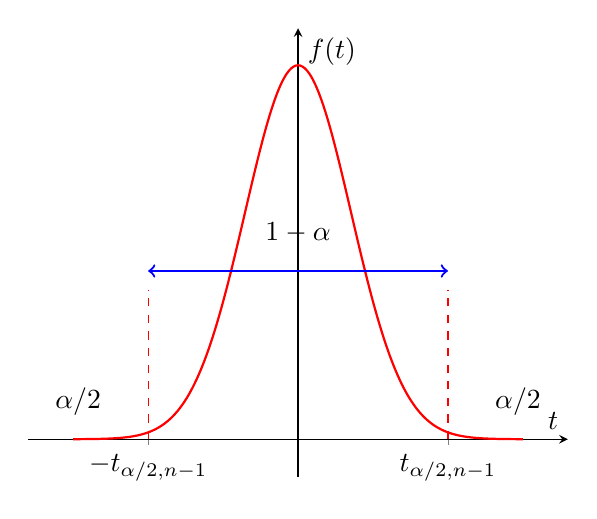
\begin{tikzpicture}
        \begin{axis}[
            axis lines=middle,
            enlargelimits=true,
            xlabel={$t$},
            ylabel={$f(t)$},
            xtick={-2, 2},
            xticklabels={$-t_{\alpha/2,n-1}$, $t_{\alpha/2,n-1}$},
            ytick=\empty,
            clip=false,
            domain=-3:3,
            samples=100,
            color=black
        ]
        \addplot [smooth, thick, red] {exp(-x^2)};
        \draw [dashed, red] (axis cs:-2,0) -- (axis cs:-2,0.4);
        \draw [dashed, red] (axis cs:2,0) -- (axis cs:2,0.4);
        \node at (axis cs:0,0.5) [above] {$1 - \alpha$};
        \node at (axis cs:-2.5,0.1) [left] {$\alpha/2$};
        \node at (axis cs:2.5,0.1) [right] {$\alpha/2$};
        \draw [<->, thick, blue] (axis cs:-2,0.45) -- (axis cs:2,0.45);
        \end{axis}
    \end{tikzpicture}
    \caption{Two sided inference with the student-t distribution.}
\end{figure}

We have seen that $\Bh\sim N(\B, \s^2(\X^\top\X)^{-1})$. Denote $(\X^\top\X)^{-1}=(e_{ij})_{i,j=1,\dots,p}$. We then have $\bh_j\sim N(\b_j, \s^2 e_{jj})$, so $\frac{\bh_j-\b_j}{\sqrt{e_{jj}}\s}\sim N(0,1)$. Since the variance is unknown, consider the statistic:
$$
    \frac{\bh_j-\b_j}{\sqrt{e_{jj}}\sh}
    =
    \frac{(\bh_j-\b_j)/\s\sqrt{e_{jj}}}{\sqrt{\frac{(n-p)\sh^2}{\s^2} / (n-p)}}.
$$
Recalling the properties of the estimators, we know that $\Bh, \sh^2$ are independent, that the numerator is $N(0,1)$-distributed and that $V=\frac{(n-p)\sh^2}{\s^2}\sim \chi^2_{n-p}$. Hence, we may conclude:
\begin{equation}
    \boxed{T = \frac{\bh_j-\b_j}{\sqrt{e_{jj}}\sh} \sim t_{n-p}}
\end{equation}
With this, we may constrict \term{confidence interval} by rewriting the inequalities in the expression:
$$
    \p{-t_{\frac{\alpha}{2},n-p} \leq \frac{\bh_j-\b_j}{\sqrt{e_{jj}}\sh} \leq t_{\frac{\alpha}{2}, n-p}} = 1-\alpha.
$$
We may also perform \term{hypothesis testing}. Consider the following test at significance level $\alpha$:
$$
    \mr{H}_0 : \b_j = 0, 
    \quad\quad\quad
    \mr{H}_1 : \b_j \ne 0.
$$
Under $H_0$ we have $T=\frac{\bh_j-\b_j}{\sqrt{e_{jj}}\sh} \sim t_{n-p}$. The \term{critical region} under two-sided alternative is:
$$
    \abs{T} \geq t_{\frac{\alpha}{2}, n-p} \Rightarrow \mr{H}_0 \textrm{ is rejected}.
$$

\TODO{R printout with explanation of culumns}

\TODO{Does R do one or two sided hypothesis test ???}

%%%%%%%%%%%%%%%%%%%%%%%%%%%%%%%%%%%%%%%%%%%%%%%%%%%%
%\subsection*{Lecture 12}
\subsection{Some notes on independence}

We sometimes use that plugging independente random variables through some functions result in new independent random variables. The theorem below tells us when this is okay. 

\begin{theorem}
    Suppose $X, Y$ are independent random variables and that $f, g$ are two measurable functions. Then $f(X), g(Y)$ are also independent. 
\end{theorem}

A \term{measurable function} is a function s.t. the preimages of Borel sets are measurable in the given probability space. In particular, continous functions are measurable.


%%%%%%%%%%%%%%%%%%%%%%%%%%%%%%%%%%%%%%%%%%%%%%%%%%%%
\subsection{Analysis of variance (ANOVA)}
The following theorem forms the basis on our discussion of ANOVA. 
\begin{theorem} \label{thm:ANOVA}
    Assuming the necesarry assumptions, we have the \term{ANOVA decomposition}:
    $$
    \boxed{
    \underset{\mr{SST}}{\underbrace{
        \sum_{i=1}^n (Y_i - \bar{Y})}} = 
    \underset{\mr{SSR}}{\underbrace{
        \sum_{i=1}^n (\hat{Y}_i - \bar{Y})}} + 
    \underset{\mr{SSE}}{\underbrace{
        \sum_{i=1}^n (Y_i - \hat{Y}_i)^2}}
    }
    $$
\end{theorem}
\begin{proof}
    We first split the sum as:
    \begin{align*}
        \sum_{i=1}^{n}\left(Y_{i}-\bar{Y}\right)^{2}
        &=\sum_{i=1}^{n}\left(Y_{i}-\hat{Y}_{i}+\hat{Y}_{i}-\bar{Y}\right)^{2}
        \\&= \sum_{i=1}^{n}\left(Y_{i}-\hat{Y}_{i}\right)^{2}+\sum_{i=1}^{n}\left(\hat{Y}_{i}-\bar{Y}\right)^2 
        +2{\sum_{i=1}^{n}\left(Y_{i}-\hat{Y}\right)\left(\hat{Y}_{i}-\bar{Y}\right)}.
    \end{align*}
    Using again the properties of the estimators, we find that the last sum is $0$:
    $$
        \sum_{i=1}^{n}\left(Y_{i}-\hat{Y}\right)\left(\hat{Y}_{i}-\bar{Y}\right)
        =
        \underbrace{\sum_{i=1}^{n} \overbrace{(Y_i-\hat{Y}_i)}^{\e_i}\hat{Y}_{i}}_{=\Eh^\top\hat{\Y}=0}
        -\bar{Y}\underbrace{\sum_{i=1}^{n}\left(Y_{i}-\hat{Y}\right)}_{=0 \textrm{ by property 2}}.
    $$
\end{proof}
The 3 sums are called \term{total sum of squares}, \term{regression sum of squares} and \term{error sum of squares} respectivelly. 
This decomposition motivates the following definition. 
\begin{definition}
    The part of the total variation due to the model is called the \term{coefficient of determination} or the \term{R2-score}:
    \begin{equation}
        \boxed{
            R^2 = \frac{\mr{SSR}}{\mr{SST}} \overset{\mr{thm}} = 1 - \frac{\mr{SSE}}{\mr{SST}}}        
    \end{equation}
\end{definition}
The R2-score is a measure of goodness-of-fit as it tells us how much of the variation in the data can be explained by the model. One may also prove another representation:
$$
    R^2 = \frac{\brac{\sum_{i=1}^n(Y_i-\bar{Y})(\hat{Y}_i-\bar{Y})}^2}{\sum_{i=1}^n(Y_i-\bar{Y})^2\sum_{i=1}^n(\hat{Y}_i-\bar{Y})}.
$$
This is the square of the empirical correlation between $\Y, \hat{\Y}$.

%%%%%%%%%%%%%%%%%%%%%%%%%%%%%%%%%%%%%%%%%%%%%%%%%%%%
%\subsection*{Lecture 13}
\subsubsection{Fictional model}
The following discussion will examine what happens when an explanatory variable is explained by the other explanatory variables. We introduce a \term{fictional model} using $x_{ij}$ as response for some fixed feature $j$. Wlog use feature $k$. The model is:
$$
    x_{i,k} = \alpha_0 + \alpha_1 x_{i,1} + \dots + \alpha_{k-1} x_{i, k-1} + \delta_i.
$$
As usual, we assume $\bs{\delta}=(\delta_1,\dots,\delta_n)^\top\sim N(0, \s^2\mI)$. We may then estimate $\bs{\alpha}=(\alpha_0,\dots,\alpha_{k-1})^\top$ and $\s^2$ by the usual $\hat{\bs{\alpha}}, \sh^2$ to obtain fitted $\hat{x}_{ik}$. We find the squared empirical correlation between $x_{i,k}$ and $\hat{x_{i,k}}$ as:
$$
    R_k^2 
    = \frac{\sum_{i=1}^n (\hat{x}_{ik}-\bar{x_k})^2}{\sum_{i=1}^n ({x}_{ik}-\bar{x_k})^2} 
    = \frac{\brac{\sum_{i=1}^n ({x}_{ik}-\bar{x_k})(\hat{x}_{ik}-\bar{x_k})}^2}
    {\sum_{i=1}^n ({x}_{ik}-\bar{x_k})^2\sum_{i=1}^n (\hat{x}_{ik}-\bar{x_k})^2}.
$$
We call it the coefficient of determination for $x_{ik}$ as response. Repeating the procedure for the remaining $x_{ij}, j=1,\dots,k-1$ we obtain $R_1^2,\dots,R_k^2$. It turns out that:
$$
    \var{\bh_j} = \frac{\s^2}{(1-R_j^2)\sum_{i=1}^n(x_{ij}-\bar{x}_j)}.
$$
So the more a variable is explained by the other, the higher the variance of the estimator.
%%%%%%%%%%%%%%%%%%%%%%%%%%%%%%%%%%%%%%%%%%%%%%%%%%%%
\subsubsection{Further expressions for the sums of squares}
Recall that $\mC, \mH$ are both symmetric an idempotent. For the total sum of squares, using that the centering matrix $\mC$ is idempotent, we obain:
\begin{align*}
    \mr{SST} = \sum_{i=1}^n(Y_i-\bar{Y})^2 = (\mC\Y)^\top(\mC\Y) = \Y^\top \mC \Y = \Y^\top\brac{\mI-\frac{1}{n}\one\one^\top}\Y.
\end{align*}
For the residual sum of squares we also need the fact that $\mH\x_i=\x_i$ for all columns of $\X$. This follows readily as $\mH\X=\X(\X^\top\X)^{-1}\X^\top\X=\X$. From this we have $\mH\one = \one$ as this is the first column of $\X$. 
\begin{align*}
    \mr{SSR} 
    &= \sum_{i=1}^n(\hat{Y}_i-\bar{Y})^2 
    = (\mC\mH\Y)^\top(\mC\mH\Y) 
    = \Y^\top\mH\mC\mH\Y 
    \\&= \Y^\top\brac{\mH-\frac{1}{n}\mH\one\one^\top\mH^\top}\Y 
    = \Y^\top\brac{\mH-\frac{1}{n}\one\one^\top}\Y.
\end{align*}
About the matrix $\mH-\frac{1}{n}\one\one^\top$, we note that it is symmetric, idempotent and of rank $p-1$:
$$
    \rank{\mH-\frac{1}{n}\one\one^\top} = \tr{\mH-\frac{1}{n}\one\one^\top} = \tr{\mH}-\frac{1}{n}\tr{\one\one^\top}=p-1.
$$
Finally, for the error sum of squares we obtain using that $\mI-\mH$ is symmetric and idempotent:
$$
    \mr{SSE} = \sum_{i=1}^n(\hat{Y}_i-Y_i)^2 = \Eh^\top\Eh = ((\mI-\mH)\Y)^\top(\mI-\mH)\Y = \dots = \Y^\top(\mI-\mH)\Y.
$$
%%%%%%%%%%%%%%%%%%%%%%%%%%%%%%%%%%%%%%%%%%%%%%%%%%%%
\subsection{F-test}
\label{sec:F_test}
We first consider the hypothesis test:
$$
    \mr{H}_0 : \b_i = 0 \quad\forall i\in\{1,\dots,k\},
    \quad\quad\quad
    \mr{H}_1 : \b_i \ne 0 \textrm{ for at least one } i\in\{1,\dots,k\}.
$$
As usual we denote the significance level by $\alpha$. Our test statistic $F$ is:
\begin{align}
    \boxed{F = \frac{\mr{SSR}/(p-1)}{\mr{SSE}/(n-p)} \sim F_{p-1,n-p}}
\end{align}
And as usual the test is $F \geq f_{\alpha, p-1,n-p} \Rightarrow \mr{H}_0$ is rejected.
\begin{proof}
    \TODO{Uke 8}
\end{proof}

%%%%%%%%%%%%%%%%%%%%%%%%%%%%%%%%%%%%%%%%%%%%%%%%%%%%
\subsection{General F-test}
We set up a much more general problem. Let $A\in\R^{r\times p}$, $r<p$, $\mathrm{rank}(A)=r$, $\boldsymbol{d}\in\R^d$. We test the hypothesis:
$$
    \mr{H}_0 : A\B = \bs{d}, 
    \quad\quad\quad
    \mr{H}_1 : A\B \ne \bs{d}.
$$
Some special cases of this general setup are.
\begin{enumerate}[label=\textbullet]
    \item $r=1, d=0, A=(0, \dots, 1, \dots, 0)$ with $1$ at index $i$, gives the test 
    $$
        \mr{H}_0 : \b_i = 0, 
        \quad\quad\quad
        \mr{H}_1 : \b_i \ne 0.
    $$
    \item $r=1, d=0, A=(0, \dots, 1, \dots, -1, \dots, 0)$ with $1$ at index $i$ and $-1$ at index $j$, gives the test 
    $$
        \mr{H}_0 : \b_i = \b_j,
        \quad\quad\quad
        \mr{H}_1 : \b_i \ne \b_j.
    $$
    \item $r=k, d=\bs{0}\in\R^k, A=(\bs{0}, \mr{diag}(1))\in\R^{k\times p}$, gives the test 
    $$
        \mr{H}_0 : \b_i = 0 \quad\forall i\in\{1,\dots,k\},
        \quad\quad\quad
        \mr{H}_1 : \b_i \ne 0 \textrm{ for some } i\in\{1,\dots,k\}.
    $$
    This is the F-test of the previous section.
\end{enumerate}
%\subsection*{Lecture 14}
Let $\mathcal{B}$ be the space of $\B$ satisfying $\mr{H}_0$. The restricted problem is:
$$
    \Bh^R = \argmin_{\B\in\mathcal{B}}(\Y-\X\B)^\top(\Y-\X\B).
$$
Using lagrange multipliers and a bag of tricks, we obtain:
$$
    \Bh^R = \Bh - (\X^\top\X)^{-1}\bs{A}^\top(\bs{A}(\X^\top\X)^{-1}\mA^\top)^{-1}(\bs{A}\Bh-\bs{d}).
$$
Denoting $\Delta = \Bh-\Bh^R$, we find:
$$
    \mr{SSE}^R = \mr{SSE} + \Delta^\top\X^\top\X\Delta
$$
We claim that the under $\mr{H}_0$, we have
\begin{equation}
    \boxed{F = \frac{\brac{\mr{SSE}^R-\mr{SSE}} / r}{\mr{SSE}/(n-p)} \sim F_{r, n-p}}    
\end{equation}
\begin{proof}
    \TODO{Uke 8}
\end{proof}

%\subsection*{Lecture 15}
%... example ...

% \begin{figure}[H]\centering
%     \begin{tikzpicture}

%         % Axis
%         \begin{axis}[
%             no markers, 
%             domain=0:5, 
%             samples=100, 
%             axis lines*=left, 
%             xlabel=$F$, 
%             ylabel={}, 
%             height=6cm, 
%             width=10cm, 
%             xtick=\empty, 
%             ytick=\empty, 
%             enlargelimits=false, 
%             clip=false, 
%             axis on top,
%             grid = major,
%             color=black
%             ]
        
%             % F-distribution curve
%             \addplot+[smooth, thick] {x^2*exp(-x)};
            
%             % Critical value line and shaded region
%             \draw[thick] (axis cs:3,0) -- (axis cs:3,0.3);
%             \fill[pattern=north east lines, pattern color=black] (axis cs:3,0) -- (axis cs:5,0) -- (axis cs:5,0.05) -- (axis cs:3,0.05) -- cycle;
        
%             % Labels
%             \node at (axis cs:4,0.15) {$\alpha$};
%             \node[above] at (axis cs:3,0.3) {$f_{x,r_1,n-p}$};
%             \node[right] at (axis cs:4,0.4) {$H_0$ rejected};
%         \end{axis}
        
%         % Additional labels and annotations
%         \node[above right] at (8,3) {$F \geq f_{x,r_1,n-p}$};
        
%         \end{tikzpicture}
% \end{figure}


%%%%%%%%%%%%%%%%%%%%%%%%%%%%%%%%%%%%%%%%%%%%%%%%%%%%
\subsection{Transformations of data}
Some models common in applications are:
\begin{enumerate}
    \item $Y=\b_0+\b_1\frac{1}{x}+\varepsilon$
    \item $Y=\frac{1}{\b_0 x + \b_1 + \e}$
    \item $Y=\frac{x}{\b_0 x + \b_1 + x\e}$
\end{enumerate}
These can also be analysed using linear regression after undergoing some \term{transformations}, namelly:
\begin{enumerate}
    \item $\tilde{x}=\frac{1}{x} \leadsto Y=\b_0+\b_1\tilde{x}+\varepsilon$
    \item $\tilde{Y}=\frac{1}{Y} \leadsto \tilde{Y}=\b_0+\b_1{x}+\varepsilon$
    \item $\tilde{x}=\frac{1}{x},\tilde{Y}=\frac{1}{Y} \leadsto \tilde{Y}=\b_0+\b_1\tilde{x}+\varepsilon$
\end{enumerate}
We do not always know what form the model should have, which motivates the following section.

%%%%%%%%%%%%%%%%%%%%%%%%%%%%%%%%%%%%%%%%%%%%%%%%%%%%
\subsubsection{Box-Cox transformation}
The \term{Box-Cox transformation} is a power transform of the form:
\begin{equation}
    \boxed{
        u_{\lambda}(y) =
        \begin{cases}
            \begin{aligned}
                &\frac{y^\lambda-1}{\lambda}, && \text{if } \lambda \ne 0, \\
                &\ln{y}, && \text{if } \lambda = 0.
            \end{aligned}
        \end{cases}        
    }
\end{equation}
We immediatelly see that this requires $\Y>0$ the response $\Y$. To remedy negative $\Y$, simply shift them. To apply the transform, suppose that $\tilde{Y} = u_{\lambda}(Y)$ is normal and choose $\lambda$ which maximises the log-likelihood function. This turns out to not have analytic solution. 
To find the optimal $\lambda$, we therefore perform a \term{grid search}. In practice, we use the R function \texttt{boxcox}. 

%%%%%%%%%%%%%%%%%%%%%%%%%%%%%%%%%%%%%%%%%%%%%%%%%%%%
\subsubsection{Variance stabilising transformation}

Suppose $\mu_i=\ev{Y_i}$ and that $\var{Y_i}$ depends on $\mu_i$ by say $\var{Y_i}=h(\mu_i)$. Our goal is to transform by $\tilde{Y} = g(Y)$ so that the variance depends less on $\mu$. First order taylor expansion of $g(Y)$ around $\mu$ gives:
$$
    g(y) \approx g(\mu) + g'(\mu)(y-\mu).
$$ 
We find:
\begin{align*}
    \ev{g(Y)} &\approx g(\mu) + g'(\mu)\overbrace{(\ev{Y}-\mu )}^{=0} = g(\mu) 
    \\
    \var{g(Y)} &\approx \var{g(\mu) + g'(\mu)(Y-\mu)} = g'(\mu)^2\var{Y} 
\end{align*}
Choose $g(y)=\int_c^y \frac{1}{\sqrt{h(\mu)}}d\mu$. Then $g'(y) = \frac{1}{\sqrt{h(y)}}$ so $\var{g(Y)} = 1$.
